\chapter{Fahrdynamik}


\section{Schaltung}

\subsubsection*{Notwendige Komponenten}
Für den Aufbau der Schaltung sind folgende Komponenten erforderlich\ref{fig:26}:

\begin{figure}[h]
    \centering
    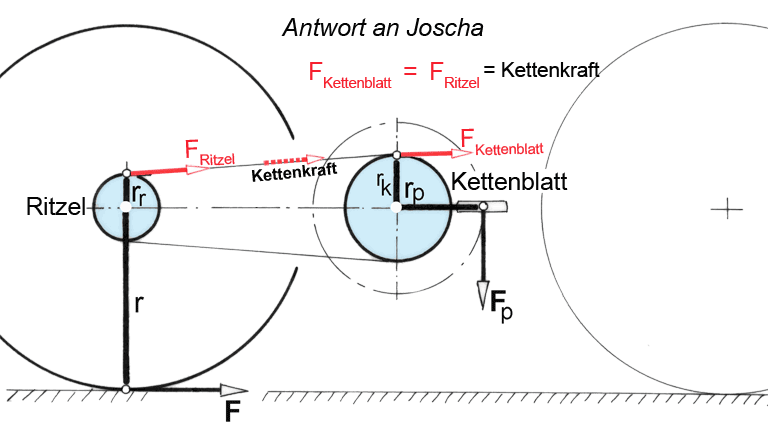
\includegraphics[width=8cm]{images/fahrrad_kraefte_gross.png}
    \caption{Fahrrad Schaltung Kraftausübung\cite{noauthor_schaltung_nodate}}%
    \label{fig:26}
\end{figure}
  

\begin{itemize}
    \item Kassette 
    \item Kettenblatt 
    \item Umwerfer
    \item Schaltwerk
    \item Schaltzüge
\end{itemize}

Der Motor hat ein Traditional Thread-on Freewheel.
Hier sind die beiden Verfahren zu sehen wie eine Kassette montiert werden kann\ref{fig:24}:

\begin{figure}[h!]
    \centering
    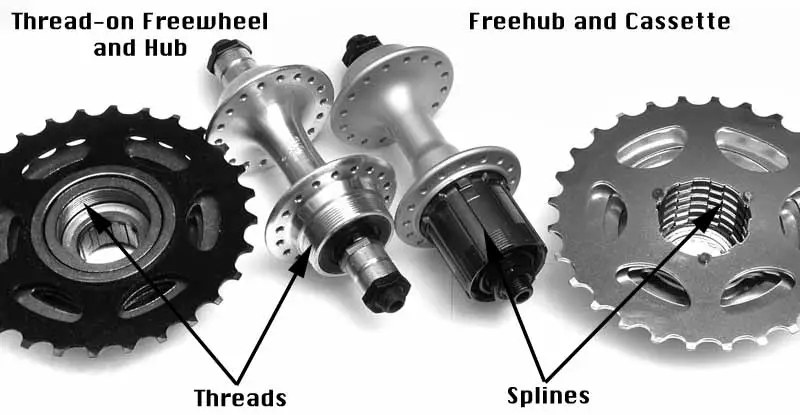
\includegraphics[width=8cm]{images/freewheel-vs-k7.png}
    \caption{Fahrrad Schaltung\cite{noauthor_traditional_nodate}}
    \label{fig:24}
\end{figure}


Bei der Auswahl der Schaltung für das selbst gebaute E-Bike ist es wichtig, die Kompatibilität zwischen dem Motor und den vorhandenen Fahrradkomponenten zu berücksichtigen.
Da der Motor einen Traditional Thread-on Freewheel-Anschluss hat \ref{fig:25}, kann der vorhandene Kassettenblock des Fahrrads nicht verwendet werden.

\begin{figure}[h]
    \centering
    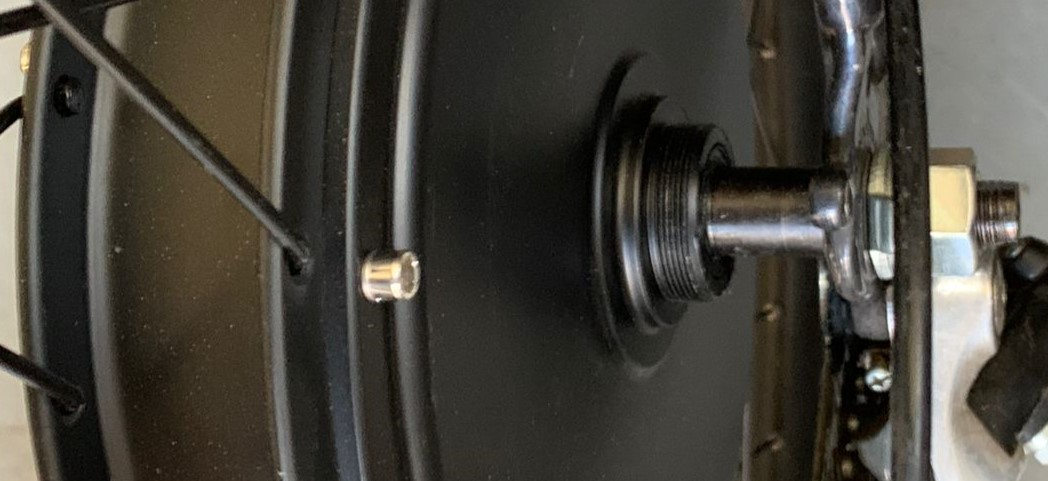
\includegraphics[width=8cm]{images/Radnabenmotoranschluss.jpg}
    \caption{Fahrradschaltung\cite{noauthor_schaltung_nodate}}
    \label{fig:25}
\end{figure}


Abgesehen von der Kassette können die vorhandenen Schaltungs-Komponenten weiterverwendet werden.

\subsubsection*{Auswahl der Kassette}
Die Kassette und das Kettenblatt beeinflussen die Geschwindigkeit und Übersetzung des E-Bikes maßgeblich.
Da eine neue Kassette benötigt wird, ist dies die erste Option, um die Übersetzung und Geschwindigkeit anzupassen.


\subsubsection*{Geschwindigkeits-Anforderungen}
Das E-Bike ist für Geschwindigkeiten zwischen 20 und 50 Stundenkilometern ausgelegt.
Daher wird ein kleines Ritzel \ref{fig:19} hinten bevorzugt, da beim Anfahren der Motor stark unterstützt und bei höheren Geschwindigkeiten weniger Widerstand benötigt wird.

% Bild des Ritzel einblenden
\begin{figure}[h]
    \centering
    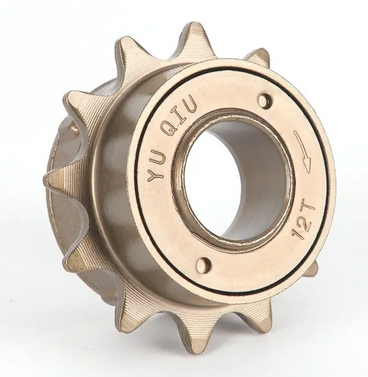
\includegraphics[width=4cm]{images/kleines Ritzel.png}
    \caption{Fahrradschaltung\cite{noauthor_423_nodate}}
    \label{fig:19}
\end{figure}

Aktuell verfügt das E-Bike über zwei Gänge durch die beiden vorhandenen Kettenblätter vorne.
Um den Motor auch bei Geschwindigkeiten über 40 Kilometer pro Stunde zu unterstützen, müssen die Kettenblätter modifiziert werden.

%\section{Fahrgefühl}



